\documentclass[conf]{new-aiaa}
%\documentclass[journal]{new-aiaa} for journal papers
\usepackage[utf8]{inputenc}

\usepackage{graphicx}
\usepackage{amsmath}
\usepackage[version=4]{mhchem}
\usepackage{siunitx}
\usepackage{placeins}
\usepackage{longtable,tabularx}
\setlength\LTleft{0pt} 

\title{Extended Abstract
Effective Use of Digital Elevation Models to Procure Ground Elevations for Flight Data}

\author{Benny Godwin Manoharan\textsuperscript{1}, Linda K. Kliment\textsuperscript{2}, Alok N. Menon\textsuperscript{3} and Kamran Rokhsaz\textsuperscript{4}}
\affil{Wichita State University, Wichita, KS 67260-0042, USA}
\let\thefootnote\relax\footnotetext{\textsuperscript{1}Student Research Assistant, Department of Aerospace Engineering, Student Member AIAA.}
\let\thefootnote\relax\footnotetext{\textsuperscript{2}Associate Professor, Department of Aerospace Engineering, Senior Member AIAA.}
\let\thefootnote\relax\footnotetext{\textsuperscript{3}Assistant Educator, Department of Aerospace Engineering, Senior Member AIAA.}
\let\thefootnote\relax\footnotetext{\textsuperscript{4}Professor Emeritus, Department of Aerospace Engineering, Associate Fellow AIAA}

\begin{document}

\maketitle

\begin{abstract}
A study was performed at Wichita State University to identify the most efficient approach to acquire ground elevations for large numbers of flight data files. There was a suite of two primary methods that were tested and assessed for their efficiency which were, Standard Application Processing Interface and using Digital Elevations models for the same purpose. The results were collected based on total time for files and time per query. The results compared favorably to Digital Elevation Models to use for mass elevation processing for flight data.
\end{abstract}

\section{Nomenclature}
{\renewcommand\arraystretch{1.0}
\noindent\begin{longtable*}{@{}l @{\quad=\quad} l@{}}
$USGS$ & United States Geological Survey \\
$DEM$ & Digital Elevation Model \\
$NTSB$ & National Transportation Safety Board \\
$DFDR$ & Digital Flight Data Recorder \\
$MSL$ & Mean Sea Level  \\
$AGL$ & Above Ground Level \\
$RMSE$ & Root Mean Squared Error \\
$TNM$ & The National Map (USGS) \\
$LMSL$ & Local Mean Sea Level \\
$USFS$ & United States Forest Service \\
$FAA$ & Federal Aviation Administration \\
$EPQS$ & Elevation Point Query Service \\
$API$ & Application Programming Interface
\end{longtable*}}

\section{Introduction}
The United States Forest Service (USFS) has a program in order to continuously monitor the health of the aircraft used in support of fire-fighting efforts.  This program was a result of in-flight failures due to fatigue.  To highlight a specific incident, a Lockheed Martin C-130A with tail number N130HP had a fatal crash in June 2002 which resulted in the loss of two lives and the aircraft. The National Transportation Safety Board Aviation Accident Final Report conclusively ascertained that the aircraft suffered fatigue failure at the center wing box beam-to-fuselage attachment location while the aircraft was maneuvered after the completion of the fire-retardant drop. This and a similar accident due to structural failure in July 2002 resulted in an extensive investigation of issues related to aerial firefighting.  As a result of this investigation and recommendations of the National Transportation Safety Board (\href{https://www.baaa-acro.com/sites/default/files/2021-03/N130HP.pdf}{NTSB}), USFS developed a program with the goal of monitoring the usage and flight loads for aircraft used in firefighting support roles.  Of particular interest are the maneuver load factors during the fire-retardant drop. As part of the flight loads monitoring program, airtankers that are operated under contract with USFS are required to have a Digital Flight Data Recorder (DFDR) and the data is made available to USFS.  The sensors are regularly calibrated, and the operators are required to record parameters defined by USFS to ensure usage information and load factors are tracked.  The aircraft operators perform their own analysis of the flight data.  In addition, an analysis is also done by researchers at Wichita State University as part of an agreement with FAA and USFS.  The primary deliverable of the analysis are the gust and maneuver load factor exceedance spectra.  Federal Aviation Administration (FAA) partners with USFS in the effort to characterize the load factor exceedance spectra for the airtankers contracted by the USFS. Due to the nature of how the aircraft is flown in USFS missions, these exceedance spectra are presented in Mean Sea Level (MSL) and Above Ground Level (AGL) altitude bands.  The necessity of defining the spectra in both altitude bands stems from the fact that the aircraft are flown very close to the ground during retardant drops, which occur at 150 ft AGL based on USFS guidance.  Therefore, the gust and maneuver load factors are shown to correlate with AGL altitudes during the phases of flight associated with the retardant drop.  In addition, AGL altitude helps in defining flight phases. 

Neither AGL altitude nor ground elevation is included in the recorded flight data, and therefore this information must be collected from other sources before completing the disclosed for load factor analysis. 

The latitude and longitude coordinates of the airplane are included as part of the recorded flight data.  Therefore, a simple query of an elevation database will return the ground elevation.  The challenge comes from the number of queries that are required, since the flight data is recorded at 32 Hz. In past studies, the National Elevation Dataset (NED) developed by US Geological Survey (USGS) was queried in order to obtain ground elevations.  However, this query method was found to be time-consuming, since there may be more than 5,000 flight hours considered during an analysis.  The study presented in this paper was conducted in order to analyze two separate methods of procuring ground elevation data.  During this study, three different services that are open to the public were used and identical information was secured from each.  The goal was to study the reliability and efficiency of each method.  

\section{Method of Analysis}
The process of acquiring elevation data for Flight data can be acquired from a variety of sources, and some of the primary solutions are listed below. For the purposes of this paper, two service providers were chosen and a total of three different product offerings were tested.

\begin{itemize} \item \textbf{Elevation Point Query Service (EPQS)} – The Elevation Point Query Service offered by the USGS was chosen for past studies due to its nature of government origin, thereby positing they provide accurate, comprehensive, and up-to-date information. Because the flight loads projects are done in partnership with USFS and FAA, using a government dataset was also desired. The data provided by USGS is collected in the 3D Elevation Program (3DEP) and is made available through an Application Programming Interface (API). The Web Coverage Service (WCS) includes multiple resolutions of Digital Elevation Models (DEM) from differing sources. For portions of the country, lidar data provides DEMs with 1 meter resolution, although this does not offer complete coverage of the continental United States.  More widespread, 1/3rd arc-second DEMs (approximately 10 m resolution) offer complete coverage of the continental US. The accuracy therefore varies based on the best source available at the location of interest. The overall accuracy of the service is currently published as being 0.53 meters Root Mean Squared Error (RMSE). It should be noted that USGS offers several query tools, including the Elevation Point Query Service, the Bulk Point Query Service, and the Spot Elevation Widget within The National Map (TNM) Viewer.  The elevations from all of these tools are based on the same datasets and algorithms. (\href{https://www.usgs.gov/faqs/how-accurate-are-elevations-generated-elevation-point-query-service-national-map}{Source}) 

\item \textbf{1/3\textsuperscript{rd} Arc Second Digital Elevation Models} – Offered by USGS, a Digital Elevation Model (DEM) is a representation of the topographic surface of the Earth excluding trees, buildings, and any other surface objects (Source). The 1/3rd arc second DEMs offer complete coverage of the United States and many of the US territories, with the exception of some parts of Alaska.  The 1/3rd-arc-second DEMs offer a resolution of approximately 10 m and were collected using a variety of sources. Elevation values are referenced to the vertical datum for the US, which was established in 1988.  (\href{https://data.usgs.gov/datacatalog/data/USGS:3a81321b-c153-416f-98b7-cc8e5f0e17c3}{Source}).

\item \textbf{Elevation Application Programming Interface (Google LLC)} – Elevation API is a service offered by Google LLC which provides elevations worldwide, or an interpolated elevation if one is not available. The interpolated elevations are based on those of the four nearest locations relative to the coordinate of interest. The ground elevations are measured relative to the Local Mean Sea Level (LMSL), which is based on an hourly average of sea levels measured over 19 years at locations across the United States. (\href{https://education.nationalgeographic.org/resource/sea-level/}{Source}). This API service has a request limit of 6,000 per minute and also requires a secure API key.

\end{itemize}

\subsection{Analysis Setup}

In order to perform this study, ten thousand random latitude and longitude pairs were generated in Python 3.12.7 in both the Continental United States (Excluding Alaska) and within the bounds of California. The points are shown in Fig. 1 and 2.  The randomly generated points were checked with a rough polygon shape for the US and likewise for California. The program also ensured no duplicate pairs. The ground elevations were then provided using each of the three methods listed above.  There were constraints in the APIs:

\begin{itemize}

    \item If an elevation was not found on the first attempt, the maximum number of retries for the APIs was set at ten.
    \item Specifically for Google LLC API, the rate limit, as per the policies, were imposed at six thousand requests per minute.

\end{itemize}

\begin{figure}[htbp]
    \centering
    \begin{minipage}{0.48\textwidth}
        \centering
        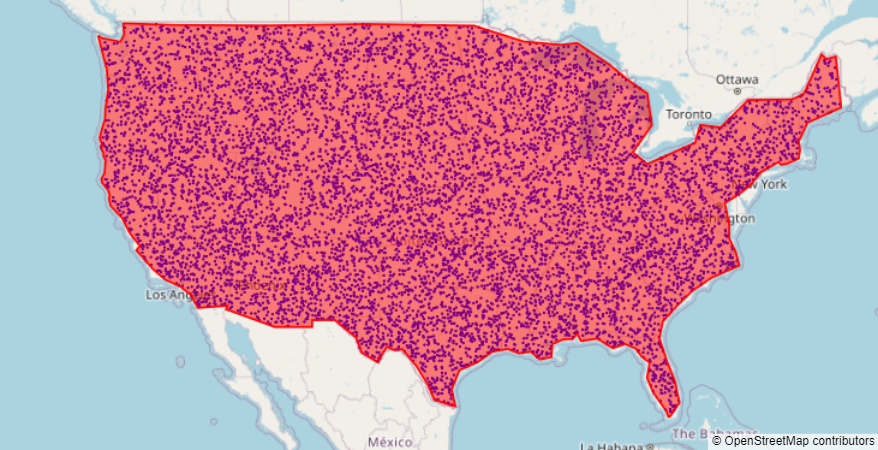
\includegraphics[width=\textwidth]{Random Points Generated in the Continental United States depicted with blue dots.png}
        \caption{Random Points Generated in the Continental United States depicted with blue dots.\href{https://www.openstreetmap.org/copyright}{Credit}}
    \end{minipage}
    \hfill
    \begin{minipage}{0.45\textwidth}
        \centering
        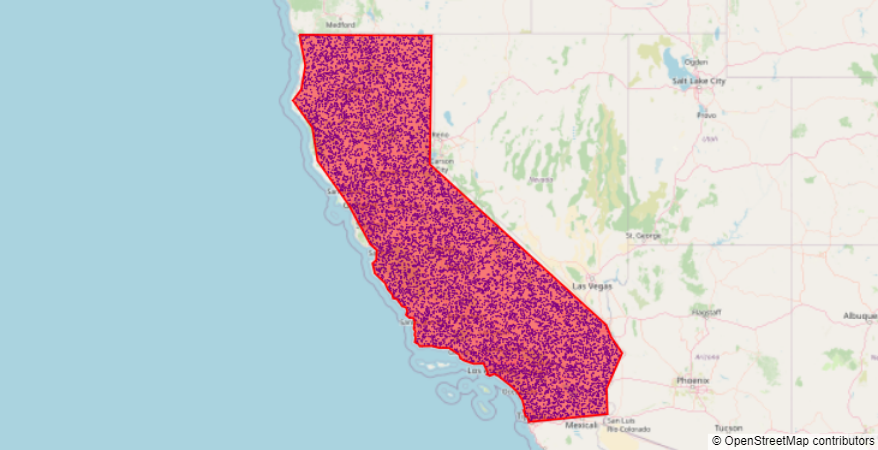
\includegraphics[width=\textwidth]{Random Points Generated in the State of California depicted with blue dots.png}
        \caption{Random Points Generated in the State of California depicted with blue dots. \href{https://www.openstreetmap.org/copyright}{Credit}}
    \end{minipage}
\end{figure}

% Fig 1. and Fig 2. show  Ten thousand random pairs of latitudes and longitudes that were generated in Python 3.12.7 in both the Continental United States (Excluding Alaska) and within the bounds of California. The randomly generated points were checked with a rough polygon shape for the US and likewise for California. The program also ensured no duplicate pairs. The points were then provided to each of the methods listed above with the following constraints in the APIs. The maximum number of retirees for the APIs was set at ten and specifically for Google, the rate limit as per the policies of Google were imposed at six thousand requests per minute.

The data collected from each of the methods included time per query and the elevation returned. Elevations returned in meters were converted to feet with a factor of 3.28084. For the APIs, the download and upload speed were measured before each query. Care was taken to measure the time per query so that it was not affected by other code operations. The python libraries used within the code are listed below. 

\begin{itemize} \item \textbf{NumPy} – A scientific computing package in Python that allows for fast mathematical processing and efficient file reading and writing. For each method, it was used to read the coordinates from a file and write out the collected elevation data in a clean format. (\href{https://numpy.org/doc/stable/}{Source}) 

\item \textbf{Pandas} – A data analysis package in Python used for managing large datasets in a simple structure known as a data frame. A data frame organizes information into a two-dimensional format of rows and columns, similar to an Excel spreadsheet.  (\href{https://pandas.pydata.org/}{Source}) 

\item \textbf{GDAL} – The Geospatial Data Abstraction Library (GDAL) is a Python package that enables the reading and processing of Digital Elevation Models (DEMs) and the extraction of geospatial information.  (\href{https://gdal.org/}{Source}) \end{itemize}

\section{Results and Discussion}

The elevations for the ten thousand points in the continental United States and the state of California were found and using the three methods described in the previous section. The results in this section are shown to make a comparison between the three methods and the strengths and weaknesses of each are discussed.

\subsection{Time Based Analysis}

The time per query is shown for the three methods in Fig. 3 for the continental United States and in Fig. 4 for California.  It should be noted that the time scale for Fig. 3 extends to 120 seconds due to one outlier.  Overall, the results in the two figures are similar, with DEM resulting in the lower times and EPQS resulting in the higher.
A summary of the graphical results is shown in Tables 2 and 3 for the continental United Stated and California, respectively.  The minimum, average, and maximum time per query are shown for each of the three methods.  The results consistently show that the lowest time is due to DEM and the highest is from EPQS.

\FloatBarrier

\begin{figure}[htbp]
    \centering
    \includegraphics[width=\textwidth]{Time Per Query (s) vs Query Index - United States Test-case.png}
    \caption{Time Per Query (s) vs Query Index - United States Test-case.}
\end{figure}

\vspace{-10pt}
\FloatBarrier

\begin{figure}[htbp]
    \centering
    \includegraphics[width=\textwidth]{Time Per Query (s) vs Query Index - California Test-case.png}
    \caption{Time Per Query (s) vs Query Index - California Test-case.}
\end{figure}

\vspace{-10pt}
\FloatBarrier

\begin{table}[htbp]
    \centering
    \begin{minipage}{.45\textwidth}
        \centering
        \caption{\label{tab:table1} Time Data Summary - United States}
        \begin{tabular}{lccc}
        \hline
        \textbf{Time For Queries} & \textbf{EPQS} & \textbf{DEM} & \textbf{Google LLC} \\
        \hline
        Minimum (s) & 0.2343 & 0.0016 & 0.0970 \\
        Average (s) & 1.0179 & 0.0193 & 0.2280 \\
        Maximum (s) & 116.9097 & 0.1568 & 15.2410 \\
        \hline
        \end{tabular}
    \end{minipage}%
    \hspace{0.06\textwidth}
    \begin{minipage}{.45\textwidth}
        \centering
        \caption{\label{tab:table2} Time Data Summary - California}
        \begin{tabular}{lccc}
        \hline
        \textbf{Time For Queries} & \textbf{EPQS} & \textbf{DEM} & \textbf{Google LLC} \\
        \hline
        Minimum (s) & 0.2264 & 0.0017 & 0.0958 \\
        Average (s) & 0.8603 & 0.0193 & 0.2450 \\
        Maximum (s) & 17.7141 & 0.0641 & 3.9179 \\
        \hline
        \end{tabular}
    \end{minipage}
\end{table}

It is clear that the DEM method results in a query time that is significantly lower than the other two methods.  This is true even with the delay due to indexing which is present with the DEM method.
As a reference to ensure that the network speed did not influence the time per query, the upload and download speeds were examined with respect to time per query.  No noticeable trend could be associated between the two as the time per query and network speed seemed to be independent of each other.  This is shown in the following figures which will be discussed in the final paper.

\begin{figure}[htbp]
    \centering
    \includegraphics[width=\textwidth]{EPQS Time Per Query vs Network Speed - US Test-case.png}
    \caption{Time Per Query (s) vs Network Speeds - EPQS - US Test-case.}
\end{figure}

\begin{figure}[htbp]
    \centering
    \includegraphics[width=\textwidth]{Google Time Per Query vs Network Speed - US Test-case.png}
    \caption{Time Per Query (s) vs Network Speeds - Google - US Test-case.}
\end{figure}

\begin{figure}[htbp]
    \centering
    \includegraphics[width=\textwidth]{EPQS Time Per Query vs Network Speed - California Test-case.png}
    \caption{Time Per Query (s) vs Query Index - EPQS - California Test-case.}
\end{figure}

\begin{figure}[htbp]
    \centering
    \includegraphics[width=\textwidth]{Google Time Per Query vs Network Speed - California Test-case.png}
    \caption{Time Per Query (s) vs Network Speeds - Google - California Test-case.}
\end{figure}

\FloatBarrier

It is clear that the DEM method results in a query time that is significantly lower than the other two methods.  This is true even with the delay due to indexing which is present with the DEM method.
As a reference to ensure that the network speed did not influence the time per query, the upload and download speeds were examined with respect to time per query.  No noticeable trend could be associated between the two as the time per query and network speed seemed to be independent of each other.  This is shown in the following figures which will be discussed in the final paper.

\subsection{Qualitative Analysis}

While time per query was a consideration, it is also important that the resulting ground elevations can be used with confidence.  Therefore, the ground elevations resulting from each method were compared.   EPQS has been used in past studies to find ground elevations and, therefore, the elevation resulting from this method was treated as the baseline.  The results in this section are presented as the difference between the baseline and DEM and Google, respectively.  
The results for the continental United States are shown in Fig. 5 and Table 4.  In a significant number of cases, the differences between EPQS and Google exceed 500 feet.   Contrary to this, there are no cases in which the difference between EPQS and DEM exceeds 60 feet.  Similar results are shown for California in Fig. 6 and Table 5, although the differences between EPQS and Google are smaller in magnitude.  

\begin{figure}[htbp]
    \centering
    \includegraphics[width=\textwidth]{Difference from EPQS - Elevations vs Query Number - US Test-case.png}
    \caption{Difference from EPQS - Elevations vs Query Number - US Test-case.}
\end{figure}

\FloatBarrier

\begin{figure}[htbp]
    \centering
    \includegraphics[width=\textwidth]{Difference from EPQS - Elevations vs Query Number - California Test-case.png}
    \caption{Difference from EPQS - Elevations vs Query Number - California Test-case.}
\end{figure}

\FloatBarrier

\begin{table}[htbp]
    \centering
    \begin{minipage}{.45\textwidth}
        \centering
        \caption{\label{tab:table1} Elevation Difference Summary - US Test-case}
        \begin{tabular}{lccc}
        \hline
        \textbf{Method} & \textbf{Minimum (ft)} & \textbf{Average (ft)} & \textbf{Maximum (ft)} \\
        \hline
        DEM & -56.4565 & 0.0247 & 45.3783 \\
        Google LLC & -1047.8204 & -4.1668 & 217.5387 \\
        \hline
        \end{tabular}
    \end{minipage}%
    \hspace{0.06\textwidth}
    \begin{minipage}{.45\textwidth}
        \centering
        \caption{\label{tab:table2} Elevation Difference Summary - California Test-case}
        \begin{tabular}{lccc}
        \hline
        \textbf{Method} & \textbf{Minimum (ft)} & \textbf{Average (ft)} & \textbf{Maximum (ft)} \\
        \hline
        DEM & -52.9620 & 0.0147 & 59.5413 \\
        Google LLC & -676.3424 & 0.0989 & 308.1487 \\
        \hline
        \end{tabular}
    \end{minipage}
\end{table}

\FloatBarrier

While the EPQS and DEM data are both offered by USGS, there is reduced fidelity in the DEM images. However, the differences between EPQS and DEM remain below 60 feet.  Contrary to this, some Google ground elevations differed significantly from the USGS methods.  On closer examination, elevations that differed by more than 200 feet were visually examined.  It was discovered that the points were mostly located within bodies of water, although a few were land regions of significant terrain changes.  Google was observed to have more accurate elevations compared to EPQS or DEM methods which can be explained due to available higher fidelity.

\FloatBarrier

\section{Conclusion}

The results clearly point to a much more time efficient DEM system to procure elevation data for flight data processing, especially for air tanker operations where loads analysis is heavily dependent on the Above Ground altitude of the aircraft. This method is not limited to this application, but rather can be used for a variety of applications both in flight data analysis and beyond, wherever the need of procuring large amounts of flight data arises.

A full conclusion will be included in the final paper.

\FloatBarrier

\section{To Be Included in the Final Paper}

For the final paper, the following items will be addressed:

\begin{itemize} \item The paper abstract and conclusion will be expanded to include results.
\item The discussions in the results section will be expanded.
\item If possible, some statistical results will also be added, including standard deviation and root mean square deviation. \end{itemize}

\FloatBarrier

% \section*{Acknowledgments}

% I would like to express my sincere thanks to Dr. Linda Kliment, Associate Professor and Associate Director of NASA in Kansas at the Department of Aerospace Engineering at Wichita State University, for her patient guidance, help and support throughout the duration of this project and her assistance and guidance in bringing this paper to fruition. I would also like to express my thanks to Dr. Alok Menon, Assistant Educator at the Department of Aerospace Engineering at Wichita State University for his help and guidance in the idea of DEMs. I also would like to acknowlegde the assistance of Dr. Kamran Rokhsaz and Dr. Alok Menon for their assistance in the analysis methods and editing of this paper.

\end{document}